%! suppress = EnDash
%! suppress = EscapeUnderscore
%! suppress = FileNotFound
Reinforcement learning lies between supervised and unsupervised learning. Namely while there is no supervision, there
is a reward for every step/ decision acting like a feedback that usually comes delayed after few steps. This makes 
time really important since we are dealing with sequential and not i.i.d data and most importantly the actions of 
the agent affect the subsequent data it receives. In other words we deal with dynamical environments with high 
dependencies. \v

The idea that we learn by interacting with our environment is probably the first to occur to us when we think about 
the nature of learning. Interactions produce a wealth of information about cause and effect, about the consequences 
of actions, and about what to do in order to achieve goals. Throughout our lives, such interactions are undoubtedly 
a major source of knowledge about our environment and ourselves. Learning from interaction is a foundational idea 
underlying nearly all theories of learning and intelligence. \v

Reinforcement learning is simultaneously a problem, a class of solution methods that work well on the class of 
problems, and the field that studies these problems and their solution methods. Reinforcement learning problems 
involve learning what to do, how to map situations to actions, so as to maximize a numerical reward signal. In an 
essential way they are closed-loop problems because the learning system's actions influence its later inputs. 
Moreover, the learner is not told which actions to take but instead must discover which actions yield the most reward
by trying them out. In the most interesting and challenging cases, actions may affect not only the immediate reward 
but also the next situation and, through that, all subsequent rewards. \v

An agent must be able to sense the state of the environment to some extent and must be able to take actions that 
affect the state. The agent also must have a goal relating to the state of the environment. The formulation is 
intended to include just these three aspects, i.e.\ sensation, action, and goal, in their simplest possible forms
without trivializing any of them. Any method that is well suited to solving this kind of problem we consider to be a 
reinforcement learning method. \v

One of the challenges that arise in reinforcement learning, and not in other kinds of learning, is the trade-off 
between exploration and exploitation. To obtain a lot of reward, a reinforcement learning agent must prefer actions 
that it has tried in the past and found to be effective in producing reward. But to discover such actions, it has to
try actions that it has not selected before. The agent has to exploit what it already knows in order to obtain 
reward, but it also has to explore in order to make better action selections in the future. The dilemma is that 
neither exploration nor exploitation can be pursued exclusively without failing at the task. The agent must try a 
variety of actions and progressively favour those that appear to be best. \v

Another key feature of reinforcement learning is that it explicitly considers the whole problem of a goal-directed 
agent interacting with an uncertain environment. This is in contrast with many approaches that consider sub-problems 
without addressing how they might fit into a larger picture. Reinforcement learning takes the opposite tack, starting
with a complete, interactive, goal-seeking agent. All reinforcement learning agents have explicit goals, can sense
aspects of their environments, and can choose actions to influence their environments. Moreover, it is usually 
assumed from the beginning that the agent has to operate despite significant uncertainty about the environment it 
faces. When reinforcement learning involves planning, it has to address the interplay between planning and real-time 
action selection, as well as the question of how environment models are acquired and improved.

\section{Basic Definitions}

\bd[Reinforcement Learning]
\textbf{Reinforcement learning} is an area of machine learning concerned with how intelligent agents ought to take 
actions in an environment in order to maximize the notion of cumulative reward. 
\ed

In simple words reinforcement learning tries to optimize a sequence of decisions. In what follows we will define the 
basic elements of reinforcement learning problems. There are a lot of definitions but they cover the entirety of all 
reinforcement learning problems.

\bd[Agent]
An \textbf{agent} is an autonomous entity which acts, directing its activity towards achieving goals upon an 
environment using observations through sensors and consequent actuators. 
\ed

An agent should, among others, accommodate new problem solving rules incrementally and adapt online and in real 
time. It should be also able to analyse itself in terms of behaviour, error and success. When it comes to learning 
it should learn quickly from large amounts of data and improve through interaction with the environment. Finally, it
should have a memory-based exemplar storage and retrieval capacities and parameters to represent short and long term 
memory.

\bd[State]
A \textbf{state} (at time $t$) $S_t$ is a representation of the current situation of an agent, or an environment.
\ed

In simple words a state is all the information an agent uses in order to determines what happens next. We distinguish
between the ``agent state'' and ``environment state''.

\bd[Agent State]
\textbf{Agent state} is the agent's internal representation.
\ed

\bd[Environment State]
\textbf{Environment state} is the environment's private (not known to agent) representation.
\ed

\bd[Action]
An \textbf{action} (at time $t$) $A_t$ is the choice of action by an agent
given a state.
\ed

\bd[Reward]
A \textbf{reward} (at time $t$) $R_t$ is an abstract concept that describes
a scalar feedback signal an agent
receives from a given state in an environment, given its action on the state.
\ed

A reward can be positive or negative. When the reward is positive, it is corresponding to our normal meaning of 
reward. When the reward is negative, it is corresponding to what we usually call ``punishment''.

\bd[Reward Hypothesis]
\textbf{Reward Hypothesis} states that all goals of an agent can be described by the maximization of an expected 
cumulative reward. 
\ed

Hence, the agent's goal is to select actions in order to maximize the future total expected cumulative reward, given
that each action might have long term consequences hence, a reward might be delayed. This makes reinforcement learning
problems quite complicated since in some cases it might be better to sacrifice an immediate reward to gain more long 
term reward. \v

We have used the term ``environment'' many times without having properly define it. At this point we have all the 
ingredients needed in order to give a definition.

\bd[Environment]
An \textbf{environment} is the entity that receives the action from an agent and emits a state and a reward.
\ed

An environment can be either ``fully observable'' or ``partially observable''.

\bd[Fully Observable Environment]
A \textbf{fully observable environment} is the case where the agent directly observes the environment state. In this 
case the agent's state and the environment's state coincide. 
\ed

\bd[Partially Observable Environment]
A \textbf{partially observable environment} is the case where the agent indirectly observes the environment state. 
In this case the agent's state is different than the environment's state and the agent must construct its own state 
representation. 
\ed

In a fully observable environment the agent receives as a state the whole environment state and it uses it as its own
state to take a decision. Fully observable environments is the main framework used in reinforcement learning since 
they constitute the vast majority of reinforcement learning problems. \v

Let's summarize the definitions we have provided so far. An agent within an environment observes an initial state 
$S_1$ it is in, and it takes an action $A_1$. The action $A_1$ is received by the environment which, by its turn, it
emits a reward $R_1$ and a new state $S_2$. The reward $R_1$ informs the agent how good the action $A_1$ was, and 
the state $S_2$ makes the agent to take a new action $A_2$, and so on. \v

\fig{rl}{0.5}

\bd[History]
\textbf{History} (at time $t$) $H_t$ is the sequence of states, actions and rewards from the very beginning up to 
time $t$:
\bse
H_t = \{S_1, A_1,R_1,S_2, A_2,R_2,\ldots, S_t, A_t,R_t \}
\ese
\ed

Moving on to some more definitions, we turn now our attention to the agent and we define the concept of a ``policy'' 
which, in a way, determines the agent's behaviour.

\bd[Policy]
A \textbf{policy} $\pi$ is a map from state space to action space and determines the behaviour of the agent in each
state:
\bse
\pi : S \to A
\ese
\ed

A policy can be either ``deterministic'' or ``stochastic''.

\bd[Deterministic Policy]
A \textbf{deterministic policy} is a policy that assigns one action $a$ to every state $s$ with probability 1:
\bse
\pi(s) = a
\ese
\ed

\bd[Stochastic Policy]
A \textbf{stochastic policy} is a policy that assigns a probability distribution over actions $a$ to every state $s$:
\bse
\pi(a|s) = P(A_t=a|S_t=s)
\ese
\ed

\bd[Policy-Based]
An agent that tries to learn an optimal policy is called \textbf{policy-based}.
\ed

Having in hand a policy one can define a quantity that ``measures'' how good this policy is. This quantity is the so 
called ``value function'' and since it measures the goodness of a specific policy, it is always attached to a 
specific policy $\pi$.

\bd[Value Function]
A \textbf{value function} $V_{\pi}$ of a policy $\pi$ is a map from state space to real numbers and it represents a 
prediction of expected future reward an agent will get by following policy $\pi$:
\bse
V_{\pi} : S \to R
\ese
\ed

A value function gives us the expected future total reward tan an agent will get if it starts form state $s$ and 
follows policy $\pi$. In general is hard to use a value function in order to realize how an agent should act. However
it is a very easy task to translate a value function to a corresponding policy and this is the reason why we always 
assign a policy to a value function.

\bd[Value-Based]
An agent that tries to learn an optimal value function is called \textbf{value-based}.
\ed

\bd[Actor-Critic]
An agent that has both a policy and a value function is called \textbf{actor-critic}.
\ed

A final, crucial part of reinforcement learning problems is the concept of a ``model'' of the environment. In general 
an agent might have a model of the environment or not. In order to define the concept of a model we first need two 
more definitions that we will also see in detail in the next chapters.

\bd[State Transition Probability]
The \textbf{state transition probability} $\mathcal{P}$ provides all the relevant information on the probability of 
an agent ending up on a successor state given that it started from an initial state. 
\ed

\bd[Expected Reward]
The \textbf{expected reward} $\mathcal{R}$ is the expected,, immediate reward an agent will get given current its 
state and action. 
\ed

Both ``state transition probability'' and ``expected reward'' will be defined again in later chapters with more detail 
and in the appropriate mathematical framework. For now we will use them to define the ``model''.

\bd[Model]
A \textbf{model} (of the environment) is a tuple $(\mathcal{P},\mathcal{R})$ where $\mathcal{P}$ is the state 
transition probability and $\mathcal{R}$ is the expected reward. 
\ed

\bd[Model-Based]
An agent that has access to a model of the environment is called \textbf{model-based}.
\ed

\bd[Model-Free]
An agent that has not access to a model of the environment is called \textbf{model-free}.
\ed

Depending on if the agent has a policy or a value function (or both) and if it also has a model or not we can end up 
in four different reinforcement learnings problems:
\bit
\item Model-Free Policy-Based
\item Model Free Value-Based
\item Model-Based Policy-Based
\item Model Based Value-Based
\eit

\bd [Planning]
In the case of model-based reinforcement learning problems where a model of the environment is known, the agent 
performs computations with its model (without any external interaction) and then it improves its policy. We refer to 
this case as \textbf{planning}. 
\ed

\bd[Reinforcement Learning (Reprise)]
In the case of model-free reinforcement learning problems where a model of the environment is initially unknown, the
agent interacts with the environment and then it improves its policy. We refer to this case as \textbf{reinforcement 
learning}. 
\ed

Reinforcement learning is like trial-and-error learning where the agent should discover a good policy from its 
experiences of the environment without losing too much reward along the way. During this process an agent can either 
``explore'' where it finds more information about the environment or ``exploit'' where it uses known information to 
maximise reward. As we already mentioned in the introduction, it is important to explore as well as exploit and that
creates the whole trade-off between exploration and exploitation. \v

As a final note, in reinforcement learning we distinguish between two situations.

\bd[Prediction]
In \textbf{prediction} one tries to evaluate a given policy.
\ed

\bd[Control]
In \textbf{control} one tries to find an optimal policy.
\ed

The general case is that we first need to solve the prediction problem in order to solve the control problem.

\section{Markov Decision Process}

Markov decision processes (MDPs) formally describe fully observable environments (i.e.\ when the current states
completely characterise the processes) for reinforcement learning problems. It is a general truth that almost all 
reinforcement learning problems can be formalised as MDPs, since partially observable environment problems can also 
be converted into MDPs. A key characteristic in what follows is the concept of ``Markov property''. Let us start by 
defining it formally.

\bd[Markov Property]
Let $\{X_i\}$ be a stochastic process. The stochastic process is said to carry the \textbf{Markov property} if and 
only if:
\bse
P(X_{n} \mid X_{n-1}, \dots, X_{1}) = P(X_{n}= \mid X_{n-1})
\ese
\ed

Markov property refers to the memoryless property of a stochastic process, since once $X_n$ is known, the rest of the
history $\{X_1, X_2, \ldots,X_{n-1}\}$ can be thrown away since $X_n$ itself contains all the information of history 
needed ($X_n$ is a sufficient statistic of the future). In other words the future is independent of the past given 
the present. Although Markov theory is a standalone mathematical theory completely independent from reinforcement 
learning, here we will focus solely on reinforcement learning and we will define everything in terms of reinforcement
learning. \v

In order to make the connection with reinforcement learning, we define the notion of a ``Markov state'' as follows.

\bd[Markov State]
A state $S_t$ is called a \textbf{Markov state} if and only if:
\bse
P(S_{t+1} \mid S_{t}, \dots, S_{1}) = P(S_{t+1} \mid S_{t})
\ese
\ed

The Markov state captures all relevant information from the history and once the state is known, the history may be 
thrown away.

\subsection{Markov Process}

Given the definition of Markov states we are now in a position to start building the mathematical framework of Markov
decision processes. The first step towards this direction is the so called ``Markov process''. In order to define it, 
we will first (re)define in detail the ``state transition probability'' which we have already introduced in the 
previous section but for the specific case of a Markov process.

\bd[State Transition Probability (For Markov Process)]
The \textbf{state transition probability} $\mathcal{P}_{s s^\prime}$ between an initial state $s$ and a successor 
state $s^\prime$ is defined as the probability of ending in state $s^\prime$ given the current state $s$:
\bse
\mathcal{P}_{s s^\prime} = P(S_{t+1}=s^\prime \mid S_{t} = s)
\ese
\ed

It is quite usual to represent the state transition probability in the form of a matrix.

\bd[State Transition Matrix (For Markov Process)]
The \textbf{state transition matrix} $\mathcal{P}$ defines transition probabilities from all states $s$ to all 
successor states $s^\prime$:
\bse
\mathcal{P} = \begin{vmatrix}
\mathcal{P}_{11} & \mathcal{P}_{12} & \ldots & \mathcal{P}_{1n} \\
\mathcal{P}_{21} & \mathcal{P}_{22} & \ldots & \mathcal{P}_{2n} \\
\vdots & \vdots & \ddots & \vdots \\
\mathcal{P}_{n1} & \mathcal{P}_{n2} & \ldots & \mathcal{P}_{nn}
\end{vmatrix}
\ese
\ed

\v

Given the state transition probability/matrix we can now define ``Markov processes''.

\bd[Markov Process]
A \textbf{Markov process} is a tuple $(\mathcal{S}, \mathcal{P}_{s s^\prime})$ where $\mathcal{S}$ is a (finite) set 
of Markov states:
\bse
\mathcal{S} = \{s_1, s_2, \ldots, s_n\}
\ese

and $\mathcal{P}_{s s^\prime}$ is the state transition probability:
\bse
\mathcal{P}_{s s^\prime} = P(S_{t+1}=s^\prime \mid S_{t} = s)
\ese
\ed

Informally a Markov process is a stochastic model describing a sequence of possible events in which the probability 
of each event depends only on the state attained in the previous event. A countably infinite sequence, in which the 
chain moves state at discrete time steps, gives a discrete-time Markov process. A continuous-time process is called a
continuous-time Markov process. \v

Markov process is named after the Russian mathematician Andrey Markov. Markov studied Markov processes in the early 
20th century, publishing his first paper on the topic in 1906. Markov processes in continuous time were discovered 
long before Andrey Markov's work in the early 20th century in the form of the Poisson process. In 1912 Henri Poincare
studied Markov chains on finite groups with an aim to study card shuffling. Other early uses of Markov chains include
a diffusion model, introduced by Paul and Tatyana Ehrenfest in 1907, and a branching process, introduced by Francis 
Galton and Henry William Watson in 1873, preceding the work of Markov. \v

Markov chains have many applications as statistical models of real-world processes, such as studying cruise control 
systems in motor vehicles, queues or lines of customers arriving at an airport, currency exchange rates and animal 
population dynamics. \v

Markov processes are the basis for general stochastic simulation methods known as Markov chain Monte Carlo, which are
used for simulating sampling from complex probability distributions, and have found application in Bayesian 
statistics, thermodynamics, statistical mechanics, physics, chemistry, economics, finance, signal processing, 
information theory and speech processing.

\bd[Terminal State]
A \textbf{terminal state} is a state where the probability of returning to itself in the next step is equal to 1.
\ed

In other words, once the Markov process lands in a terminal state then it is over, since it cannot ``escape'' this 
state.

\bd[Episode]
An \textbf{episode} is any sequence of states of a Markov process that starts from an initial state and terminates at
a final terminal state. 
\ed

While a Markov process is a good start, at the same time is not adequate enough for describing reinforcement 
learning problems since it lacks many of the ingredients we introduced earlier for the reinforcement learning problem. 
We will now add some more complexity to a Markov process to end up in the so called ``Markov reward process''.

\subsection{Markov Reward Process}

A Markov Reward Process is similar to a Markov Process in the sense that it extends the model by adding a reward rate
to each state. An additional variable records the reward accumulated up to the current time. Hence, a Markov Reward
Process is a Markov Process with some extra ingredients. \v

These extra ingredients are the ``expected reward'' (which we have already introduced in the previous section, but we
will redefine it here adjusted for the specific case of a Markov decision process) and the so called ``discount 
factor''.

\bd[Expected Reward (For Markov Reward Process)]
\textbf{Expected reward} $\mathcal{R}_{s}$ of a state $s$ is the expected, immediate reward an agent will get for 
being in state $s$:
\bse
\mathcal{R}_{s} = E[R_{t+1} | S_t=s]
\ese
\ed

The expected reward of a state is simply the reward a state provides just for being in the state. We can verify 
mathematically that the definition is actually consistent by making use of the law of conditional expected value we 
introduced in the probability notes:
\begin{align*}
\mathcal{R}_{s} &= E[R_{t+1} | S_t=s] \\
&= \sum_{s^\prime} E[R_{t+1} | S_t=s, S_{t+1} = s^\prime] \cdot P(S_{t+1} = s^\prime | S_t = s) \\
&= \sum_{s^\prime} E[R_{t+1} | S_{t+1} = s^\prime] \cdot P_{s s^\prime} \\
&= \sum_{s^\prime} R_{s} \cdot P_{s s^\prime} \\
&= R_{s} \sum_{s^\prime} P_{s s^\prime} \\
&= R_{s}
\end{align*}

\bd[Discount Factor]
\textbf{Discount factor} $\gamma$ is a scalar quantity with $\gamma \in [0,1]$ used to discount future rewards.
\ed

In simple words discount factor is used to compute the present value of future rewards. Now that we have introduced 
the expected reward and the discount factor we can expand the notion of a Markov process to that of a Markov reward 
process.

\bd[Markov Reward Process]
A \textbf{Markov reward process} is a tuple $(\mathcal{S}, \mathcal{P}_{s s^\prime}, \mathcal{R}_{s}, \gamma)$ 
where $\mathcal{S}$ is a (finite) set of Markov states:
\bse
\mathcal{S} = \{s_1, s_2, \ldots, s_n\}
\ese

$\mathcal{P}_{s s^\prime}$ is the state transition probability:
\bse
\mathcal{P}_{s s^\prime} = P(S_{t+1}=s^\prime \mid S_{t} = s)
\ese

$\mathcal{R}_{s}$ is the expected reward:
\bse
\mathcal{R}_{s} = E[R_{t+1} | S_t=s]
\ese

and $\gamma$ is the discount factor with:
\bse
\gamma \in [0,1]
\ese
\ed

Once we have a Markov reward process we can define the concept of ``return'' as follows.

\bd[Return]
\textbf{Return} $G_t$ is the total discounted reward from time-step $t$ and forward:
\bse
G_t = R_{t+1} + \gamma R_{t+2} + \gamma^2 R_{t+3} + \ldots = \sum_{k=0}^{\infty} \gamma^k R_{t+k+1}
\ese
\ed

A few comments about the definition of return and the choice of including a discount factor in the definition are in 
order. Notice that for the discount factor holds:
\bse
\gamma \in [0,1] \Rightarrow \gamma^k \to 0 \text{\:\: as \:\:} k \to \infty
\ese

In other words the discount factor weights more the near future and less the distant future. This is why the discount
factor acts as the present value of future rewards. In general most Markov reward (and decision) processes are 
discounted. This is happening for many reasons. First of all it is mathematically convenient to discount rewards. 
Secondly we avoid infinite returns in cyclic Markov processes. Thirdly, uncertainty about the future may not be fully
represented. Finally, animal/human behaviour shows preference for immediate rewards. \v

In one extreme case where only the immediate reward is important we can set $\gamma = 0$ and then we simply obtain 
$G_t = R_{t+1}$. This is called ``myopic'' evaluation. It is also possible to use undiscounted Markov reward processes
$\gamma = 1$ where all future rewards contribute equally. This is called ``far-sighted'' evaluation. In most of the 
cases we pick a value for $\gamma$ between those extreme cases. \v

Given the return $G_t$ we can now (re)define the ``state value function'' which we have already introduced in the 
previous section but for the specific case of a Markov decision process.

\bd[State Value Function (For Markov Reward Process)]
The \textbf{state value function } $V(s)$ of a Markov reward process is the total expected return an agent will 
receive starting from state $s$:
\bse
V(s) = E [G_t | S_t = s]
\ese
\ed

In simple words, state value function informs us about the expected return an agent will obtain by starting from a 
state $s$, by taking the expected value over all possible episodes that start from state $s$. Notice that in the 
case of myopic evaluation ($\gamma=0$) the value state function is equal to the expected reward since this is the 
only state that counts in any episode (for $\gamma=0$):
\bse
V(s) = E [G_t | S_t = s] = E [R_{t+1} | S_t = s] = \mathcal{R}_{s}
\ese

For values of $\gamma$ different than 0 the state value function takes into account future expected rewards as well. \v

We can manipulate the value function in order to decompose it into two parts: the expected reward and the discounted 
state value function of all possible successor states as follows:
{\setlength{\jot}{10pt}
\begin{align*}
V(s) &= E [G_t | S_t = s] \\
&= E [R_{t+1} + \gamma R_{t+2} + \gamma^2 R_{t+3} + \ldots | S_t = s] \\
&= E [R_{t+1} + \gamma (R_{t+2} + \gamma R_{t+3} + \ldots) | S_t = s] \\
&= E [R_{t+1} + \gamma G_{t+1} | S_t = s] \\
&= E [R_{t+1}| S_t = s] + E[\gamma G_{t+1} | S_t = s] \\
&= \mathcal{R}_{s} + \gamma E[G_{t+1} | S_t = s]
\end{align*}}

\vspace{-10pt}

Where in the last equality we used the definition of the reward function $\mathcal{R}_{s}$. By using the law of 
conditional expected value (check probability notes for details) we obtain:
\bse
V(s) = \mathcal{R}_{s} + \gamma \sum_{s^\prime} E[G_{t+1} | S_t = s, S_{t+1} = s^\prime] 
\cdot P(S_{t+1} = s^\prime | S_t = s)
\ese

Finally, by using the Markov property and the definition of state transition probability:
{\setlength{\jot}{10pt}
\begin{align*}
V(s) &= \mathcal{R}_{s} + \gamma \sum_{s^\prime} E[G_{t+1} | S_{t+1} = s^\prime] \cdot \mathcal{P}_{ss^\prime} \\
&= \mathcal{R}_{s} + \gamma \sum_{s^\prime} \mathcal{P}_{ss^\prime} V(s^\prime)
\end{align*}}

\vspace{-10pt}

This final expression is called ``Bellman expectation equations'' and it is used to derive the state value function 
for all states of a Markov reward process. It states that the expected return for a state $s$ (aka the state value 
function) is equal to the expected immediate reward of state $s$ plus the expected rewards of all successive states 
weighted by the probability of reaching them and discounted by $\gamma$.

\fig{rl4}{0.6}

By defining the following vectors:
\bse
\boldsymbol{V} = \begin{bmatrix} V(s_1) \\[1ex] V(s_2) \\[1ex] \vdots \\[1ex] V(s_n) \end{bmatrix}, \qquad
\boldsymbol{\mathcal{R}} = \begin{bmatrix} \mathcal{R}_{s_1} \\[1ex] \mathcal{R}_{s_2} \\[1ex] \vdots \\[1ex] 
\mathcal{R}_{s_n} \end{bmatrix}
\ese

\vspace{2pt}

we can write Bellman expectation equations in a matrix form as:
\bse
\boldsymbol{V} = \boldsymbol{\mathcal{R}} + \gamma \mathcal{P} \boldsymbol{V}
\ese

where $\mathcal{P}$ is the state transition matrix. \v

Since the equation is linear we can solve it directly (as we did in the case of Normal equation in supervised 
learning) and obtain a solution for $\boldsymbol{V}$. Namely:
{\setlength{\jot}{5pt}
\begin{align*}
& \boldsymbol{V} = \boldsymbol{\mathcal{R}} + \gamma \mathcal{P} \boldsymbol{V} \Rightarrow \\
& \boldsymbol{V} - \gamma \mathcal{P} \boldsymbol{V} = \boldsymbol{\mathcal{R}} \Rightarrow \\
& (I - \gamma \mathcal{P}) \boldsymbol{V} = \boldsymbol{\mathcal{R}} \Rightarrow \\
& (I - \gamma \mathcal{P})^{-1} (I - \gamma \mathcal{P}) \boldsymbol{V} =
(I - \gamma \mathcal{P})^{-1} \boldsymbol{\mathcal{R}} \Rightarrow \\
& \boldsymbol{V} = (I - \gamma \mathcal{P})^{-1} \boldsymbol{\mathcal{R}}
\end{align*}}

\vspace{-12pt}

As in supervised learning with normal equation, when the number of states $n$ is large the matrix $\mathcal{P}$ gets
large and computing the inverse of it, is computationally very expensive (and in some cases even impossible). \v

One of the main goals of reinforcement learning is to come up with algorithms of solving Bellman expectation
equations indirectly. We will come back to this once we have developed the full framework needed for reinforcement
learning problems. \v

Now we are ready to introduce the next and final model in this chain of complexity called ``Markov Decision Process''. 
\v

Before we move on however, let's see a detailed application of what we have discussed so far.

\subsubsection*{Application: Markov Process \& Markov Reward Process}

Let's begin with an example of a Markov process.

\fig{rl1}{0.3}

In this example the set of Markov states is:
\bse
\mathcal{S} = \{s_1, s_2, s_3, s_4, s_5, s_6, s_7\}
\ese

and the state transition matrix (we use the state transition matrix since it's more handy) is: \v

\begingroup
\renewcommand*{\arraystretch}{1.5}
\bse
\mathcal{P} = \begin{vmatrix}
0 & 0.5 & 0 & 0 & 0 & 0.5 & 0 \\
0 & 0 & 0.8 & 0 & 0 & 0 & 0.2 \\
0 & 0 & 0 & 0.6 & 0.4 & 0 & 0 \\
0 & 0 & 0 & 0 & 0 & 0 & 1 \\
0.2 & 0.4 & 0.4 & 0 & 0 & 0 & 0 \\
0.1 & 0 & 0 & 0 & 0 & 0.9 & 0 \\
0 & 0 & 0 & 0 & 0 & 0 & 1 \\
\end{vmatrix}
\ese
\endgroup

\vspace{10pt}

In this specific example the state $s_7$ is a terminal state, hence, a possible episode could be:
\bse
S_1=s_1, \to S_2=s_2, \to S_3=s_3, \to S_4=s_4, \to S_5=s_7
\ese

Now let's see how can we turn this to a Markov Reward Process.

\fig{rl2}{0.3}

As we can see, the only difference with the Markov process is that now in Markov decision process each state carries
a reward $R$. \v

As a practice on the concept of the return one could compute the return of the episode we mentioned in the previous
example:
\bse
S_1=s_1, \to S_2=s_2, \to S_3=s_3, \to S_4=s_4, \to S_5=s_7
\ese

By choosing $\gamma=0.5$ we have:
\begin{align*}
G_1 &= \sum_{k=0}^{\infty} 0.5^k R_{1+k+1} \\
&= (0.5)^0 R_{2} +(0.5)^1 R_{3} + (0.5)^2 R_{4} + (0.5)^3 R_{5} \\
&= (1) (-2) + (0.5) (-2) + (0.25) (-2) + (0.125) (10) \\
& = -2.25
\end{align*}

In order to practise more, let's calculate the state value functions for the states using the the Bellman expectation
equations. \v

In the extreme case where $\gamma=0$ we already showed that:
\bse
V(s) = \mathcal{R}_{s} + (0) \sum_{s^\prime} \mathcal{P}_{s s^\prime} V(s^\prime) = \mathcal{R}_{s}
\ese

Hence, in the myopic evaluation, the state value functions are equal to the immediate expected rewards of each state,
no matter what the agent will do after that.

\fig{rl3}{0.4}

In the case where $\gamma$ is different than zero, one has to take into account future expected rewards on top of the
immediate expected reward. For example for the first state $s_1$, for $\gamma=0.9$ it is:

{\setlength{\jot}{5pt}
\begin{align*}
V(s_1) &= \mathcal{R}_{s_1} + 0.5 \sum_{s^\prime} \mathcal{P}_{s_1 s^\prime} V(s^\prime) \\
&= -2 + 0.9 (\mathcal{P}_{s_1 s_1} V(s_1) + \mathcal{P}_{s_1 s_2} V(s_2) + \mathcal{P}_{s_1 s_3} V(s_3) +
\mathcal{P}_{s_1 s_4} V(s_4) + \mathcal{P}_{s_1 s_5} V(s_5) + \mathcal{P}_{s_1 s_6} V(s_6) +
\mathcal{P}_{s_1 s_7} V(s_7) \\
&= -2 + 0.9 ((0) V(s_1) +(0.5) V(s_2) +(0)V(s_3) + (0) V(s_4) + (0) V(s_5) + (0.5) V(s_6) + (0) V(s_7) \\
&= -2 + 0.45 V(s_2) +0.45 V(s_6)
\end{align*}}

\vspace{-10pt}

Similarly we calculate the corresponding equations for all states and then we solve the system of equations to obtain
the actual values of the state value functions. The final results are summarized below.

\fig{rl5}{0.6}

Once again, a Markov reward process is not adequate enough for describing reinforcement learning problems since there
is no notion of actions that an agent can take. We will now add a final piece of complexity to a Markov reward
process by introducing ``action'' to end up in the so called ``Markov decision process''.

\subsection{Markov Decision Process}

In mathematics, a Markov decision process (MDP) is a discrete-time stochastic control process. It provides a
mathematical framework for modeling decision making in situations where outcomes are partly random and partly under
the control of a decision maker. MDPs are useful for studying optimization problems solved via dynamic programming.
MDPs were known at least as early as the 1950s, a core body of research on Markov decision processes resulted from
Ronald Howard's 1960 book, Dynamic Programming and Markov Processes. They are used in many disciplines, including
robotics, automatic control, economics and manufacturing. The name of MDPs comes from the Russian mathematician
Andrey Markov as they are an extension of Markov chains. \v

Markov decision processes (MDPs) can be used to mathematically describe the vast majority of reinforcement learning
problems and this is why they are so useful. The starting point is the concept of an ``action'' as it was introduced
earlier, i.e.\ an action $A_t$ is an action taken by an agent at a state $S_t$ at time $t$. In reinforcement learning
we always make the assumption that at each state the agent has a finite amount of possible actions it can perform.
Once we have defined the actions we can now alter a bit the definitions of state transition probability and expected
reward in order to incorporate actions.

\bd[State Transition Probability (For Markov Decision Process)] The \textbf{state transition probability}
$\mathcal{P}_{s s^\prime}^{a}$ between an initial state $s$ and a successor state $s^\prime$ given an action $a$ is
defined as the probability of ending in state $s^\prime$ given the current state $s$ and action $a$:
\bse
\mathcal{P}_{s s^\prime}^{a} = P(S_{t+1}=s^\prime \mid S_{t} = s, A_t=a)
\ese
\ed

\bd[Expected Reward (For Markov Decision Process)]
\textbf{Expected reward} $\mathcal{R}_{s}^{a}$ of a state $s$ and action $a$ is the expected, immediate reward an
agent will get for being in state $s$ and taking the action $a$:
\bse
\mathcal{R}_{s}^{a} = E[R_{t+1} | S_t=s]
\ese
\ed

Having these definitions we can now define a ``Markov decision process''.

\bd[Markov Decision Process]
A \textbf{Markov decision process} is a tuple $(\mathcal{S}, \mathcal{A}, \mathcal{P}_{s s^\prime}^{a},
\mathcal{R}_{s}^{a}, \gamma)$ where $\mathcal{S}$ is a (finite) set of Markov states:
\bse
\mathcal{S} = \{s_1, s_2, \ldots, s_n\}
\ese

$\mathcal{A}$ is a (finite) set of actions:
\bse
\mathcal{A} = \{a_1, a_2, \ldots, a_n\}
\ese

$\mathcal{P}_{s s^\prime}^{a}$ is the state transition probability:
\bse
\mathcal{P}_{s s^\prime}^{a}= P(S_{t+1}=s^\prime \mid S_{t} = s, A_t=a)
\ese

$\mathcal{R}_{s}^{a} $ is the expected reward:
\bse
\mathcal{R}_{s}^{a} = E[R_{t+1} | S_t=s, A_t=a]
\ese

and $\gamma$ is the discount factor with:
\bse
\gamma \in [0,1]
\ese
\ed

At this point it is clear what a (stochastic) policy really is. Recall the definition of a (stochastic) policy:
\bse
\pi(a|s) = P(A_t=a|S_t=s)
\ese

Thus, a policy is really a distribution over actions given states and it fully defines the behaviour of an agent. In
other words it is in our control and not in environment's control. In MDPs policies depend on the current state and
not the history due to the Markov property. In other words policies are stationary (time-independent). \v

Now that we have a policy in hand, it is the agent who decides which action it will take and not the environment
(although in real life problems it can be a combination of both). Hence, now we will update the concept of the state
value function by substituting the expected value over state transition probability to the expected value over policy.

\bd[State Value Function (For Markov Decision Process)]
The \textbf{state value function } $V_{\pi}(s)$ of a Markov decision process is the total expected return an agent
will receive starting from state $s$ and then following policy $\pi$:
\bse
V_{\pi}(s) = E_{\pi} [G_t | S_t = s]
\ese
\ed

On top of that, in the case of MDPs we can also define a quantity similar to state value function called ``action
value function'' that incorporates the concept of action as follows.

\bd[Action Value Function]

The \textbf{action value function } $Q_{\pi}(s, a)$ of a Markov decision process is the total expected return an
agent will receive starting from state $s$, taking action $a$ and then following policy $\pi$:
\bse
Q_{\pi}(s, a)= E_{\pi} [G_t | S_t = s, A_t=a]
\ese
\ed

The two quantities, state and action value function are inner-related and we can derive the one from the other by
making use of the law of conditional expected value and the Markov property. Namely:
\begin{align*}
V_{\pi}(s) &= E_{\pi} [G_t | S_t = s] \\
&= \sum_{a} E_{\pi} [G_t | S_t = s, A_t=a] \cdot P(A_t=a \mid S_t=s) \\
&= \sum_{a} \pi(a \mid s) \cdot Q_{\pi}(s, a)
\end{align*}

What this equation really tells us is that being at state $s$ we will perform some action a with probability given by
the policy $\pi(a \mid s)$. For each action $a$, there is an action value function $Q_{\pi}(s, a)$ that says how good
the action $a$ is. Looking one step ahead, by averaging all the actions $V_{\pi}(s)$ tells us how good is it being at
state $s$, given the actions we can perform. \v

\fig{rl6}{0.6}

Similarly for the action value function:
\begingroup
\allowdisplaybreaks
{\setlength{\jot}{10pt}
\begin{align*}
Q_{\pi}(s, a) &= E_{\pi} [G_t | S_t = s, A_t=a] \\
&= E_{\pi} [R_{t+1} + \gamma R_{t+2} + \gamma^2 R_{t+3} + \ldots | S_t = s, A_t=a] \\
&= E_{\pi} [R_{t+1} + \gamma (R_{t+2} + \gamma R_{t+3} + \ldots) | S_t = s, A_t=a] \\
&= E_{\pi} [R_{t+1} + \gamma G_{t+1} | S_t = s, A_t=a] \\
&= E_{\pi} [R_{t+1}| S_t = s, A_t=a] + E_{\pi} [\gamma G_{t+1} | S_t = s, A_t=a] \\
&= \mathcal{R}_{s}^{a} + \gamma \sum_{s^\prime} E_{\pi} [G_{t+1} | S_t = s, A_t=a, S_{t+1} = s^\prime]
\cdot P(S_{t+1} = s^\prime | S_t = s, A_t=a) \\
&= \mathcal{R}_{s}^{a} + \gamma \sum_{s^\prime} E_{\pi} [G_{t+1} | S_{t+1} = s^\prime]
\cdot P(S_{t+1} = s^\prime | S_t = s, A_t=a) \\
&= \mathcal{R}_{s}^{a} + \gamma \sum_{s^{\prime}} \mathcal{P}_{s s^\prime}^{a} V_{\pi}(s^\prime)
\end{align*}}
\endgroup

where in the second last from the end line we used the Markov property to discard both $S_t = s,$ and $A_t=a$. What
this equation really tells us is that being at state $s$ we take action $a$, and the environment will return us some
immediate reward $\mathcal{R}_{s}^{a}$ and a state $s$ with probability given by $\mathcal{P}_{s s^\prime}^{a}$. For
each of these states there is a function $V_{\pi}(s^\prime)$ that says how good is the state we ended up. Looking one
step ahead by averaging all the states, $Q_{\pi}(s, a)$ tells us how good is it being at state $s$ to take action $a$.
\v

\fig{rl7}{0.6}

\vspace{-10pt}

So we showed that indeed the two quantities are related. The first one shows the expected return of starting at state
$s$ and follow policy $\pi$ why do the latter shows the expected return of starting at state $s$, take action $a$ and
then follow policy $\pi$. \v

Given an MDP our goal is to determine either the state value function or the action value function for all states and
actions. As in the case of an MRP this can be done through Bellman expectation equations that we will now derive for
both quantities. \v

Starting with the state value function:
\begingroup
\allowdisplaybreaks
{\setlength{\jot}{10pt}
\begin{align*}
V_{\pi}(s) &= E_{\pi} [G_t | S_t = s] \\
&= E_{\pi} [R_{t+1} + \gamma R_{t+2} + \gamma^2 R_{t+3} + \ldots | S_t = s] \\
&= E_{\pi} [R_{t+1} + \gamma (R_{t+2} + \gamma R_{t+3} + \ldots) | S_t = s] \\
&= E_{\pi} [R_{t+1} + \gamma G_{t+1} | S_t = s] \\
&= E_{\pi} [R_{t+1}| S_t = s] + E_{\pi} [\gamma G_{t+1} | S_t = s] \\
&= \sum_{a} E_{\pi} [R_{t+1}| S_t = s, A_t=a] \cdot P(S_{t+1} = s^\prime | S_t = s, A_t=a) + \\
& \qquad \qquad \qquad \qquad \qquad \qquad \qquad + \sum_{a} \gamma E_{\pi} [G_{t+1} | S_t = s, A_t=a]
\cdot P(S_{t+1} = s^\prime | S_t = s, A_t=a) \\
&=\sum_{a} \mathcal{R}_{s}^{a} \cdot \pi(a \mid s) + \gamma \sum_{a} E_{\pi} [G_{t+1} | S_t = s, A_t=a]
\cdot \pi(a \mid s) \\
&= \sum_{a} \mathcal{R}_{s}^{a} \cdot \pi(a \mid s) + \gamma \sum_{a} \pi(a \mid s) \sum_{s^\prime} E_{\pi}
[G_{t+1} | S_t = s, A_t=a, S_{t+1} = s^\prime ] \cdot P(S_{t+1} = s^\prime | S_t = s, A_t=a) \\
&=\sum_{a} \mathcal{R}_{s}^{a} \cdot \pi(a \mid s) + \gamma \sum_{a} \pi(a \mid s) \sum_{s^\prime} E_{\pi}
[G_{t+1} | S_{t+1} = s^\prime ] \cdot P(S_{t+1} = s^\prime | S_t = s, A_t=a) \\
&=\sum_{a} \mathcal{R}_{s}^{a} \cdot \pi(a \mid s) + \gamma \sum_{a} \pi(a \mid s) \sum_{s^\prime}
\mathcal{P}_{ss^\prime}^{a} \cdot V_{\pi}(s^\prime) \\
&=\sum_{a} \pi(a \mid s) \Big[\mathcal{R}_{s}^{a} + \gamma \sum_{s^\prime} \mathcal{P}_{ss^\prime}^{a}
\cdot V_{\pi}(s^\prime) \Big]
\end{align*}}
\endgroup

\v

What this equation tells us is how good is it being in a state $s$, to take an action $a$ based on a policy $\pi$
which, based on the state transition probability of the environment, will lead to a successor state $s^\prime$. We do
that by taking the immediate reward and then averaging out over all possible actions and all possible successor states.
\v

\fig{rl8}{0.6}

\v

Notice that the same equation can be derived by using the relations of the connection between the state and action
value functions. Namely, by substituting:
\bse
Q_{\pi}(s, a) = \mathcal{R}_{s}^{a} + \gamma \sum_{s^{\prime}} \mathcal{P}_{s s^\prime}^{a} V_{\pi}(s^\prime)
\ese

to:
\bse
V_{\pi}(s) = \sum_{a} \pi(a \mid s) \cdot Q_{\pi}(s, a)
\ese

we straight forwardly get:
\begin{align*}
V_{\pi}(s) &= \sum_{a} \pi(a \mid s) \cdot Q_{\pi}(s, a) \\
&=\sum_{a} \pi(a \mid s) \Big[\mathcal{R}_{s}^{a} +
\gamma \sum_{s^\prime} \mathcal{P}_{ss^\prime}^{a} \cdot V_{\pi}(s^\prime) \Big]
\end{align*}

Finally, for the Bellman expectation equations of the action value function we can again start from the definition and
derive them, however we can derive them much simpler by following the same trick as above, a.k.a.\ by substituting:
\bse
V_{\pi}(s) = \sum_{a} \pi(a \mid s) \cdot Q_{\pi}(s, a)
\ese

to:
\bse
Q_{\pi}(s, a) = \mathcal{R}_{s}^{a} + \gamma \sum_{s^{\prime}} \mathcal{P}_{s s^\prime}^{a} V_{\pi}(s^\prime)
\ese

By doing so we end up with:
\begin{align*}
Q_{\pi}(s, a) &= \mathcal{R}_{s}^{a} + \gamma \sum_{s^{\prime}} \mathcal{P}_{s s^\prime}^{a} V_{\pi}(s^\prime) \\
&= \mathcal{R}_{s}^{a} + \gamma \sum_{s^{\prime}} \mathcal{P}_{s s^\prime}^{a}
\sum_{a^\prime} \pi(a^\prime \mid s^\prime) \cdot Q_{\pi}(s^\prime, a^\prime)
\end{align*}

which is the Bellman expectation equation for the action value function. \v

What this equation tells us is how good is it being in a state $s$ and take an action $a$ to move to a successor
state $s^\prime$, based on the state transition probability of the environment, and then take action $a^\prime$ based
on a policy $\pi$. We do that by taking the immediate reward and then averaging out over all possible successor
states and successor actions. \v

\fig{rl9}{0.6}

\section{Optimal Policies}

As we have seen so far and MDP is all we need in order to formulate a reinforcement learning problem. Then, by having
a policy $\pi$ we can evaluate how good it is by using the Bellman expectation equations and compute either the state
or the action value functions. However, in reinforcement learning we are not interested in finding the state or the
action value function for a random policy $\pi$, rather than finding an optimal policy $\pi$ whatever that means. \v

So, it is clear that we need to find a way to define and compute an optimal policy. In order to do so we will start
with some more definitions about optimal value functions which specify the best possible performance of an MDP over
all possible policies.

\bd[Optimal State Value Function] The \textbf{optimal state value function} $V_{*}(s)$ is the maximum state value
function over all policies:

\bse
V_{*}(s) = \max_{\pi} V_{\pi}(s), \: \forall s
\ese
\ed

\bd[Optimal Action Value Function] The \textbf{optimal action value function} $Q_{*}(s,a)$ is the maximum action
state value function over all policies:
\bse
Q_{*}(s,a) = \max_{\pi} Q_{\pi}(s,a), \: \forall s,a
\ese
\ed

Once an optimal action value function $Q_{*}(s,a)$ is known, the MDP is actually solved since given any state $s$ we
know which action is the best.

\bd[Optimal Policy]
The \textbf{optimal policy} $\pi_{*}$ is the policy that generates both the optimal state value function $V_{*}(s)$
and the optimal action value function $Q_{*}(s,a)$.
\ed

Hence, for the optimal policy holds:
\bse
\pi_{*}(a \mid s)=\Big\{ \begin{array}{lr} 1, \:\: \text{ if } a =\argmax_{a} Q_{*}(s,a) \\ 0, \:\: \text{ otherwise}
\end{array}
\ese

One can prove a theorem that states:
\bit
\item There exists a policy that is better than or equal to all other policies:
\bse
\exists \pi_{*} : \pi_{*} \geq \pi \:\:\: (\text{a.k.a.\: \:} V_{\pi_{*}} (s) \geq V_{\pi}(s),
\forall s \: \text{\:\: and \:\:} \: Q_{\pi_{*}}(s,a) \geq Q_{\pi}(s,a), \forall s,a)
\ese

\item All optimal policies achieve the same optimal value functions:
\bse
V_{\pi_{*}}(s) = V_{*}(s), \forall \pi_{*} \text{\:\: and \:\:} Q_{\pi_{*}}(s,a) = Q_{*}(s,a), \forall \pi_{*}
\ese

\item There is always a deterministic optimal policy for any MDP\@.
\eit

The optimal value functions are, of course, related to each other in the same way the value functions were related to
each other. Recall that for the state value function we had:
\bse
V_{\pi}(s) = \sum_{a} \pi(a \mid s) \cdot Q_{\pi}(s, a)
\ese

For the optimal state value function holds:
\bse
V_{*}(s) = \max_{a} Q_{*}(s, a)
\ese

For the action value function we showed that:
\bse
Q_{\pi}(s, a) = \mathcal{R}_{s}^{a} + \gamma \sum_{s^{\prime}} \mathcal{P}_{s s^\prime}^{a} V_{\pi}(s^\prime)
\ese

For the optimal action value function holds:
\bse
Q_{*}(s, a) = \mathcal{R}_{s}^{a} + \gamma \sum_{s^{\prime}} \mathcal{P}_{s s^\prime}^{a} V_{*}(s^\prime)
\ese

Finally, the optimal value functions are recursively related by the Bellman optimality equations in contrast to
Bellman expectation equations that we used for the value functions. We can derive them very simply by doing the trick
of substituting the one to each other in the above relations. By doing so for the optimal state value the Bellman
optimality equations are:
\bse
V_{*}(s) = \max_{a} \left[ \mathcal{R}_{s}^{a} + \gamma \sum_{s^{\prime}}
\mathcal{P}_{s s^\prime}^{a} V_{*} (s^\prime) \right]
\ese

while for the action value function:
\bse
Q_{*}(s, a) = \mathcal{R}_{s}^{a} + \gamma \sum_{s^{\prime}}
\mathcal{P}_{s s^\prime}^{a} \max_{a^\prime} Q_{*} (s^\prime, a^\prime)
\ese

Notice that Bellman optimality equations, in contrast with Bellman expectation equations, are non-linear and most
importantly they have no closed form solutions. For this reason we need to develop some iterative solution methods
able to solve the maximization problem. This is the goal of the next chapter.

\section{Solving Markov Decision Processes}

In reality, reinforcement learning is all about developing iterative algorithms able to solve the non linear Bellman
optimality equations. In this chapter we will focus on ways to solve the Bellman expectation and optimality equations. 
Recall from the introduction that we are distinguishing between ``model-based'' scenarios where the agent has access
to a model of the environment hence, it performs computations with it in order to improve its policy (planning), and
``model-free'' scenarios where the agent has not access to a model of the environment. Recall also that we
distinguished between ``prediction'' where the agent tries to evaluate a given policy and ``control'' where the agent
tries to find an optimal policy. \v

In this chapter, eventually, we will explore all these areas! We will begin with model-based prediction and
model-based control cases in order to gain some intuition on how things work and then we will move on to the real
world full reinforcement learning problems of model free prediction and model free control cases. Let's start.

\subsection{Model-Based Prediction}

In the model-based cases (both for prediction and control) we will focus on dynamical programming. The term dynamical
programming refers to a collection of algorithms that can be used to compute optimal policies given a perfect model
of the environment as an MDP. The term ``dynamical'' refers to a sequential or temporal component of the problem.
Dynamical programming is a method for solving complex problems by breaking them into sub-problems, solving them, and
then combining them back to obtain the total solution. Given the recursive nature of Bellman equations, dynamical
programming uses the recursion as a way to divide the problem to smaller problems.

\subsubsection{Policy Evaluation}

Focusing on model-based prediction we will develop only one model called ``policy evaluation''. The way it works is
through iterative applications of Bellman expectation equation:
\bse
V_{\pi}(s) = \sum_{a} \pi(a \mid s) \Big[\mathcal{R}_{s}^{a} + \gamma \sum_{s^\prime} \mathcal{P}_{ss^\prime}^{a}
\cdot V_{\pi}(s^\prime) \Big]
\ese

(Recall that we are on the prediction case that we want to evaluate a given policy and not to derive an optimal
policy, so we don't need Bellman optimality equation) \v

As a first step, we will create a temporal series of of state value vectors:
\bse
V_0(s), V_1(s), \ldots
\ese

and by randomly initializing $V_0(s)$ to some initial values (e.g.\ by setting 0 to all entries):
\bse
V_0(s_1) = V_0(s_2) = \ldots = V_0(s_n)=0
\ese

we will then use Bellman expectation equation as an update rule to obtain $V_1(s)$ as:
\bse
V_{1}(s) = \sum_{a} \pi(a \mid s) \Big[\mathcal{R}_{s}^{a} + \gamma \sum_{s^\prime} \mathcal{P}_{ss^\prime}^{a}
\cdot V_{0}(s^\prime) \Big]
\ese

Similarly we will get $V_2(s)$ by using Bellman expectation equation as an update rule:
\bse
V_{2}(s) = \sum_{a} \pi(a \mid s) \Big[\mathcal{R}_{s}^{a} + \gamma \sum_{s^\prime} \mathcal{P}_{ss^\prime}^{a}
\cdot V_{1}(s^\prime) \Big]
\ese

The general update rule is of course:
\bse
V_{k+1}(s) = \sum_{a} \pi(a \mid s) \Big[\mathcal{R}_{s}^{a} + \gamma \sum_{s^\prime} \mathcal{P}_{ss^\prime}^{a}
\cdot V_{k}(s^\prime) \Big]
\ese

One can show, although we will skip the proof for now, that after many iterations the final state value function will
be the state value function of the policy:
\bse
V_k(s) \to V_{\pi}(s) \:\: \text{as} \:\: k \to \infty
\ese

\be
Let us give an example with the following small gridworld. We assume an undiscounted MDP ($\gamma = 1$). We have 14
non-terminal states $1, \ldots, 14$ and two terminal states shown as shaded squares. The reward is $-1$ for every
state until a terminal state is reached. The agent follows a uniform random policy:
\bse
\pi(\text{north}|\text{any state}) = \pi(\text{west}|\text{any state}) = \pi(\text{south}|\text{any state})
= \pi(\text{east}|\text{any state}) = 0.25
\ese

\fig{rl10}{0.5}

Let's see the state value function for all states after $k$ iterations. The final step $k=\infty$ is the actual
values of the evaluation of the policy ($V_\infty = V_\pi$)

\vspace{-10pt}

\begin{figure}[H]
\centering
\subfloat{{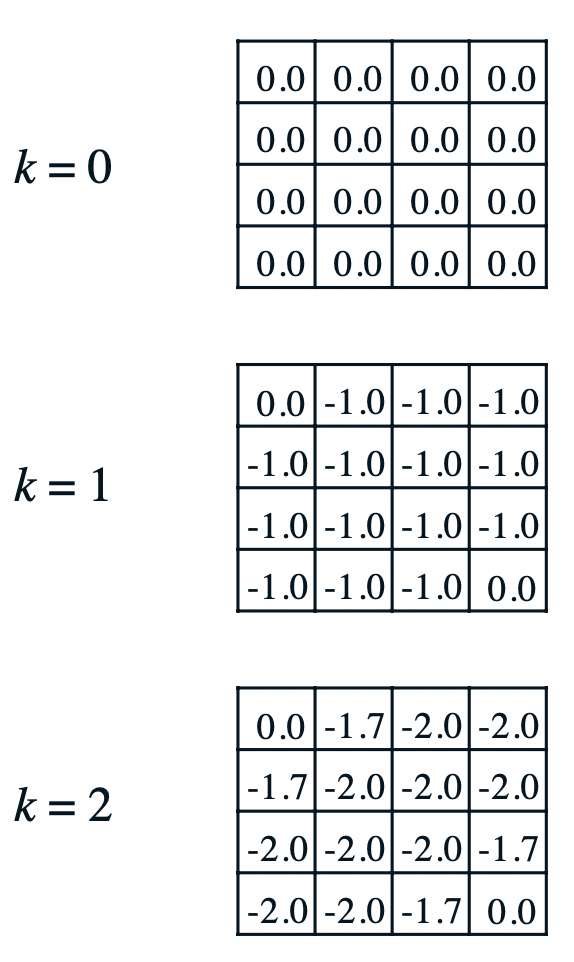
\includegraphics[width=5cm]{rl11}}}
\qquad \qquad
\subfloat{{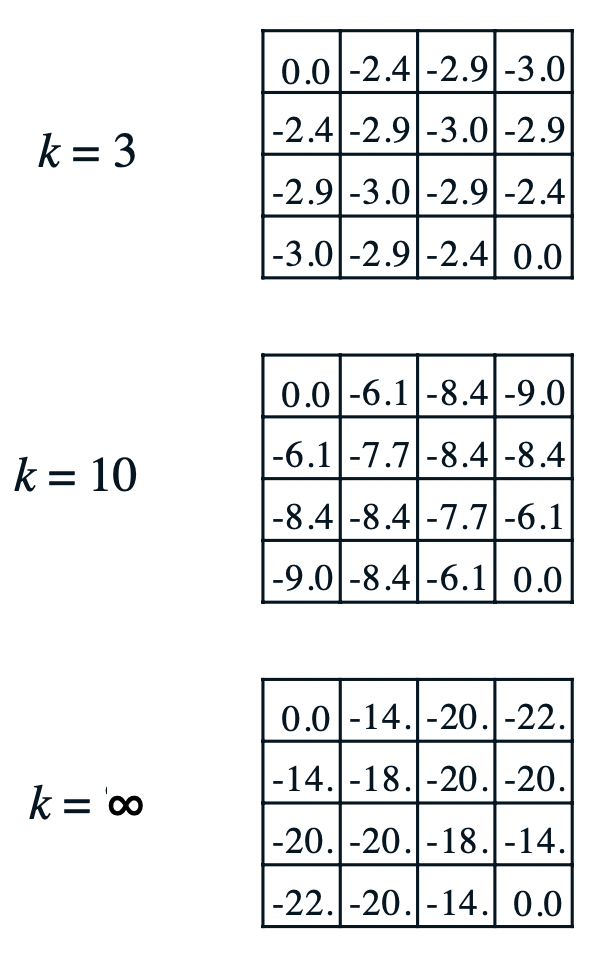
\includegraphics[width=5.25cm]{rl12}}}
\end{figure}
\ee

\subsection{Model-Based Control}

Moving on to model-based control, the task in hand now is given an MDP to find an optimal policy $\pi_{*}$. In
model-based control, we will develop two algorithms called ``policy iteration'' and ``value iteration''.

\subsubsection{Policy Iteration}

In policy evaluation we saw that given a policy $\pi$, we can initialize a set of initial state value functions $V_0
(s),$ and by making use of the Bellman expectation equation as an update rule, through an iterative process of
updates to finally evaluate the policy $\pi$. Now we can get one step further. The idea is that once we have
evaluated the policy and we have obtained the state value function $V_{\pi} (s)$, we can now update our policy $\pi$
to a new one $\pi^\prime$ by simply picking that action that maximizes the action state value function:

\bse
\pi^\prime(s) = \argmax_{a} \left[ \mathcal{R}_{s}^{a} + \gamma \sum_{s^{\prime}} \mathcal{P}_{s s^\prime}^{a}
V_{\pi}(s^\prime) \right] = \argmax_{a} Q_\pi(s,a)
\ese

Then we can start evaluating this new policy $\pi^\prime$ from the beginning. Once it is evaluated we then repeat
the same process of policy evaluation and once we have evaluated the new policy $\pi^\prime$ and we know the state
value function $\boldsymbol{V}_{\pi^\prime}$ we again update our policy $\pi^{\prime}$ to $\pi^{\prime\prime}$ as:
\bse
\pi^{\prime\prime}(s) = \argmax_{a} \left[\mathcal{R}_{s}^{a} + \gamma \sum_{s^{\prime}} \mathcal{P}_{s s^\prime}^{a}
V_{\pi^\prime}(s^\prime) \right] = \argmax_{a} Q_{\pi^\prime}(s,a)
\ese

We repeat this cycle until we reach a point of no further improvement.

\vspace{3pt}

\fig{rl18}{0.4}

One can prove that after a number of such pairs of ``evaluation-improvement'' iterations one will end up in an optimal
policy $\pi_*$.

\fig{rl17}{0.3}

Notice that in policy iteration we actually have two sets of iterations:
\bit
\item We iterate over the cycle of evaluation - improvement of policy iteration.
\item We iterate over $k$ cycles of updates through Bellman expectation equation for each evaluation of policy
evaluation.
\eit

And this is actually the major drawback of policy iteration. Every time we switch to a new policy we need to start
the evaluation straight from the beginning which is computationally expensive. This is something that we address with
the so called ``value iteration'' algorithm.

\subsubsection{Value Iteration}

Let's start by getting some intuition from the small grid world example we developed in policy evaluation.

\be
Recall that we started with all initial state values, set by us, to 0 and a uniform random policy with chance 0.25
moving anywhere.

\fig{rl13}{0.5}

After just one single iteration of the evaluation process, we ended up in $V_1 $.

\fig{rl14}{0.5}

The state value function $V_1(s)$ is certainly not the $V_{\pi}(s)$, however recall that in control we want to find
the optimal policy and not to evaluate one. Hence, nothing is stopping us from doing an update of the policy right
now, after just one step instead of waiting until the very end of the evaluation. (More generally, one can pick any
number of $k$ evaluation iterations before doing the update. This is usually called ``modified policy iteration'' or
``generalized policy iteration''. In the extreme case where $k=1$ and we do the update immediately after just one step
of evaluation iteration, the algorithm is called ``value iteration'').
\ee

Hence, in value iteration instead of moving on to the second iteration of the evaluation process of the same initial
policy $\pi$ we instead update the policy, right after the very first step of the evaluation, to a new policy
$\pi^\prime$. This update is actually happening to the state value function by making use of the Bellman optimality
equation. (Notice that this is exactly the same to the the update we do in policy iteration once the evaluation is
over):
\bse
V_{k+1} (s) \gets \max_{a} \left[ \mathcal{R}_{s}^{a} + \gamma \sum_{s^{\prime}} \mathcal{P}_{s s^\prime}^{a} V_k
(s^\prime) \right]
\ese

One can prove that after many iterations this process will lead us to an optimal state value function. Of course, for
the optimal state value function the Bellman optimality equation is true:
\bse
V_{*} (s) = \max_{a} \left[ \mathcal{R}_{s}^{a} + \gamma \sum_{s^{\prime}} \mathcal{P}_{s s^\prime}^{a} V_*
(s^\prime) \right]
\ese

Notice that for the optimal state value function we do not update ($\gets$) but verify ($=$). Once the optimal state
value function $V_*(s)$ is know, we can compute the optimal action value function:
\bse
Q_{*}(s, a) = \mathcal{R}_{s}^{a} + \gamma \sum_{s^{\prime}} \mathcal{P}_{s s^\prime}^{a} V_{*}(s^\prime)
\ese

and then the optimal policy is simply:
\bse
\pi_*(s) = \argmax_{a} Q_*(s,a)
\ese

Notice that in value iteration we now have only one set of iterations since we do not run $k$ cycles of updates
through Bellman expectation equation for each evaluation of policy evaluation but instead we update the state value
function directly after each iteration using the Bellman optimality equation.

\subsubsection*{Application: Value Iteration}

Since value iteration is very important in what follows we will examine in detail an application of an MDP solved via
value iteration. Consider the following MDP: $(\mathcal{S}, \mathcal{A}, \mathcal{P}_{s s^\prime}^{a},
\mathcal{R}_{s}^{a}, \gamma)$.

\vspace{-10pt}

\fig{rl19}{0.3}

\vspace{-10pt}

The MDP consists of 2 states $(\mathcal{S} = \{s_1, s_2\})$ and in each state the agent can perform two actions $
(\mathcal{A} = \{a_1, a_2\})$. The environment emits the following state transition probabilities:
\bse
\mathcal{P}^{a_1}_{s_1 s_1} = 0.5, \qquad \mathcal{P}^{a_1}_{s_1 s_2} = 0.5, \qquad \mathcal{P}^{a_1}_{s_2 s_1} = 0,
\qquad \mathcal{P}^{a_1}_{s_2 s_2} = 1
\ese

\bse
\mathcal{P}^{a_2}_{s_1 s_1} = 0, \qquad \mathcal{P}^{a_2}_{s_1 s_2} = 1, \qquad \mathcal{P}^{a_2}_{s_2 s_1} = 1,
\qquad \mathcal{P}^{a_2}_{s_2 s_2} = 0
\ese

\v

and the following expected rewards:
\bse
\mathcal{R}^{a_1}_{s_1} = 3, \qquad \mathcal{R}^{a_1}_{s_2} = -1, \qquad \mathcal{R}^{a_2}_{s_1} = 3,
\qquad \mathcal{R}^{a_2}_{s_2} = -1
\ese

Finally, the MDP carries a discount factor of $\gamma = 0.5$. \v

We want to find what the optimal way for an agent to behave in this MDP. We will use value iteration to find the
optimal policy. We begin by initializing $V_0 (s)$ to 0 $\forall s$, a.k.a.\:
\bse
V_0 (s_1) = 0 \qquad V_0 (s_2) = 0
\ese

Now we use the Bellman optimality equation for updating the state value function:
\bse
V_1 (s) \gets \max_{a} \left[ \mathcal{R}_{s}^{a} + \gamma \sum_{s^{\prime}} \mathcal{P}_{s s^\prime}^{a} V_0
(s^\prime) \right]
\ese

Namely for $s_1$:
\bse
V_1 (s_1) \gets \max_{a} \left[ \mathcal{R}_{s_1}^{a} + 0.5 \sum_{s^{\prime}} \mathcal{P}_{s_1 s^\prime}^{a} V_0
(s^\prime) \right]
\ese

Using $V_0 (s) = 0, \:\: \forall s$:
\bse
V_1 (s_1) \gets \max_{a} \left[ \mathcal{R}_{s_1}^{a} \right] = \max \left[ \mathcal{R}_{s_1}^{a_1},
\mathcal{R}_{s_1}^{a_2} \right] = \max \left[ 3, 3 \right] = 3
\ese

Similarly for $s_2$:
\vspace{-10pt}
{\setlength{\jot}{5pt}
\begin{align*}
V_1 (s_2) &\gets \max_{a} \left[ \mathcal{R}_{s_2}^{a} +
\gamma \sum_{s^{\prime}} \mathcal{P}_{s_2 s^\prime}^{a} V_0 (s^\prime) \right] \\
& = \max_{a} \left[ \mathcal{R}_{s_2}^{a} \right] \\
& = \max \left[ \mathcal{R}_{s_2}^{a_1}, \mathcal{R}_{s_2}^{a_2} \right] \\
& = \max \left[ -1, -1 \right] \\
& = -1
\end{align*}}

\vspace{-10pt}

Hence, after the first iteration of value iteration:
\bse
V_1 (s_1) = -3 \qquad V_1 (s_2) = -1
\ese

Moving on to the second iteration:
{\setlength{\jot}{10pt}
\begin{align*}
V_2 (s_1) & \gets \max_{a} \left[ \mathcal{R}_{s_1}^{a} +
0.5 \sum_{s^{\prime}} \mathcal{P}_{s_1 s^\prime}^{a} V_1 (s^\prime) \right] \\
& = \max \left[ \mathcal{R}_{s_1}^{a_1} + 0.5 \left( \mathcal{P}_{s_1 s_1}^{a_1} V_1 (s_1) +
\mathcal{P}_{s_1 s_2}^{a_1} V_1 (s_2) \right), \mathcal{R}_{s_1}^{a_2} +
0.5 \left( \mathcal{P}_{s_1 s_1}^{a_2} V_1 (s_1) + \mathcal{P}_{s_1 s_2}^{a_2} V_1 (s_2) \right) \right] \\
& = \max \left[ 3 + 0.5 \left( (0.5) (3) + (0.5) (-1) \right), 3 + 0.5 \left( (0) (3) + (1) (-1) \right) \right] \\
& = \max \left[ 3.5, 2.5 \right] \\
& = 3.5
\end{align*}}

\vspace{-30pt}

{\setlength{\jot}{10pt}
\begin{align*}
V_2 (s_2) & \gets \max_{a} \left[ \mathcal{R}_{s_2}^{a} + 0.5 \sum_{s^{\prime}}
\mathcal{P}_{s_2 s^\prime}^{a} V_1 (s^\prime) \right] \\
& = \max \left[ \mathcal{R}_{s_2}^{a_1} + 0.5 \left(\mathcal{P}_{s_2 s_1}^{a_1} V_1 (s_1) +
\mathcal{P}_{s_2 s_2}^{a_1} V_1 (s_2) \right), \mathcal{R}_{s_2}^{a_2} +
0.5 \left( \mathcal{P}_{s_2 s_1}^{a_2} V_1 (s_1) + \mathcal{P}_{s_2 s_2}^{a_2} V_1 (s_2) \right) \right] \\
& = \max \left[ -1 + 0.5 \left( (0) (3) + (1) (-1) \right), -1 + 0.5 \left( (1) (3) + (0) (-1) \right) \right] \\
& = \max \left[ -1.5, 0.5 \right] \\
& = 0.5
\end{align*}}

\vspace{-10pt}

Hence, after the second iteration of value iteration:
\bse
V_2 (s_1) = 3.5 \qquad V_2 (s_2) = 0.5
\ese

Similarly we move on to further iterations. Here are the values we obtain:
\bse
\boldsymbol{V}_0 = (0,0), \qquad \boldsymbol{V}_1 = (3, -1), \qquad \boldsymbol{V}_2 = (3.5, 0.5), \qquad
\boldsymbol{V}_3 = (4, 0.75)
\ese

\bse
\boldsymbol{V}_4 = (4.2, 1), \qquad \boldsymbol{V}_5 = (4.3, 1.1), \qquad \boldsymbol{V}_6 = (4.4, 1.2), \qquad
\boldsymbol{V}_7 = (4.4, 1.2)
\ese

\v

As we can see $\boldsymbol{V}_6 = \boldsymbol{V}_7$ which means that the value iteration provides no further
improvement, hence, $\boldsymbol{V}_6$ is the optimal policy. One can verify this by using now the Bellman optimality
equation not as an update rule, but as an equation the optimal state value function must satisfy. Indeed:

{\setlength{\jot}{10pt}
\begin{align*}
V_6 (s_1) & = \max_{a} \left[ \mathcal{R}_{s_1}^{a} +
0.5 \sum_{s^{\prime}} \mathcal{P}_{s_1 s^\prime}^{a} V_6 (s^\prime) \right] \\
& = \max \left[ \mathcal{R}_{s_1}^{a_1} + 0.5 \left( \mathcal{P}_{s_1 s_1}^{a_1} V_6 (s_1) +
\mathcal{P}_{s_1 s_2}^{a_1} V_6 (s_2) \right), \mathcal{R}_{s_1}^{a_2} +
0.5 \left(\mathcal{P}_{s_1 s_1}^{a_2} V_6 (s_1) + \mathcal{P}_{s_1 s_2}^{a_2} V_6 (s_2) \right) \right] \\
& = \max \left[ 3 + 0.5 \left( (0.5) (4.4) + (0.5) (1.2) \right), 3 + 0.5 \left( (0) (4.4) + (1) (1.2) \right) \right] \\
& = \max \left[ 4.4, 3.6 \right] \\
& = 4.4
\end{align*}}

\vspace{-30pt}

{\setlength{\jot}{10pt}
\begin{align*}
V_6 (s_2) & = \max_{a} \left[ \mathcal{R}_{s_2}^{a} + 0.5 \sum_{s^{\prime}} \mathcal{P}_{s_2 s^\prime}^{a}
V_6 (s^\prime) \right] \\
& = \max \left[ \mathcal{R}_{s_2}^{a_1} +
0.5 \left(mathcal{P}_{s_2 s_1}^{a_1} V_6 (s_1) + \mathcal{P}_{s_2 s_2}^{a_1} V_6 (s_2) \right),
\mathcal{R}_{s_2}^{a_2} + 0.5 \left( \mathcal{P}_{s_2 s_1}^{a_2} V_6 (s_1) +
\mathcal{P}_{s_2 s_2}^{a_2} V_6 (s_2) \right) \right] \\
& = \max \left[ 3 + 0.5 \left( (0) (4.4) + (1) (1.2) \right), 3 + 0.5 \left( (1) (4.4) + (0) (1.2) \right) \right] \\
& = \max \left[ -0.4, 1.2 \right] \\
& = 1.2
\end{align*}}

Hence, through value iteration we found the optimal state value function:
\bse
\boldsymbol{V}_* = (4.4, 1.2)
\ese

Moving on, for the optimal action value function holds:
\bse
Q_{*}(s, a) = \mathcal{R}_{s}^{a} + \gamma \sum_{s^{\prime}} \mathcal{P}_{s s^\prime}^{a} V_{*}(s^\prime)
\ese

Hence, for $s_1$:
\begin{align*}
Q_{*}(s_1, a_1) & = \mathcal{R}_{s_1}^{a_1} + 0.5 \left(\mathcal{P}_{s_1 s_1}^{a_1} V_{*}(s_1) +
\mathcal{P}_{s_1 s_2}^{a_1} V_{*}(s_2) \right) \\
& =3 + 0.5 \left((0.5) (4.4) + (0.5) (1.2) \right) \\
& = 4.4
\end{align*}

\vspace{-15pt}

\begin{align*}
Q_{*}(s_1, a_2) & = \mathcal{R}_{s_1}^{a_2} + 0.5 \left(\mathcal{P}_{s_1 s_1}^{a_2} V_{*}(s_1) +
\mathcal{P}_{s_1 s_2}^{a_2} V_{*}(s_2) \right) \\
& = 3 + 0.5 \left((0) (4.4) + (1) (1.2) \right) \\
& = 3.6
\end{align*}

Similarly for $s_2$:
\begin{align*}
Q_{*}(s_2, a_1) & = \mathcal{R}_{s_2}^{a_1} + 0.5 \left(\mathcal{P}_{s_2 s_1}^{a_1} V_{*}(s_1) +
\mathcal{P}_{s_2 s_2}^{a_1} V_{*}(s_2) \right) \\
& = -1 + 0.5 \left((0) (4.4) + (0.5) (1) \right) \\
& = -0.75
\end{align*}

\vspace{-15pt}

\begin{align*}
Q_{*}(s_2, a_2) & = \mathcal{R}_{s_2}^{a_2} + 0.5 \left(\mathcal{P}_{s_2 s_1}^{a_2} V_{*}(s_1) +
\mathcal{P}_{s_2 s_2}^{a_2} V_{*}(s_2) \right) \\
& = -1 + 0.5 \left((1) (4.4) + (0.5) (0) \right) \\
& = 1.2
\end{align*}

And now we know the action value function. Recall that we said that once we know the action value function the MDP is
solved since we know how to behave. Indeed, by following:
\bse
\pi_*(s) = \argmax_{a} Q_*(s,a)
\ese

we have:
\begin{align*}
\pi_*(s_1) &= \argmax_{a} Q_*(s_1,a) \\
&= \argmax_{a} [Q_*(s_1,a_1), Q_*(s_1,a_2)] \\
&= \argmax_{a} [4.4, 3.6] \\
&= a_1
\end{align*}

\vspace{-15pt}

\begin{align*}
\pi_*(s_2) &= \argmax_{a} Q_*(s_2,a) \\
&= \argmax_{a} [Q_*(s_2,a_1), Q_*(s_2,a_2)] \\
&= \argmax_{a} [-0.75, 1.2] \\
&= a_2
\end{align*}

Hence, the optimal way for the agent to behave is to take action $a_1$ when in state $s_1$ and action $a_2$ when in
state $s_2$.

\subsection{Model-Free Prediction}

In this chapter we will be dealing with the real reinforcement learning problem. Up to this point the MDP was fully
given. In real world problems however this is really unrealistic, since some of the entities of an MDP might be
unknown to us (mostly state transition probabilities since they are the ones controlled by the environment). \v

Hence, our goals in model-free problems are:
\bit
\item To estimate the value functions of an unknown MDP given a policy $\pi$ (model-free prediction) without knowing
how the environment might behave.
\item To optimize the value functions of an unknown MDP, and subsequently find the optimal policy $\pi_*$ (model-free
control) without knowing how the environment might behave.
\eit

We will follow the same procedure as before. We will begin with evaluating a given policy $\pi$ within an unknown MDP
(prediction) and by gaining some intuition of the problem we will move on finding optimal policies for unknown MDPs
(control). In this chapter we will deal with model-free prediction and we will analyse three algorithms: ``Monte
Carlo'', ``Temporal Difference'' and ``TD($\lambda$)''.

\subsubsection{Monte Carlo}

Monte Carlo is a model-free algorithm that learns directly from episodes of experience without bootstrapping, i.e.\
from complete episodes. This makes Monte Carlo able to be applied only to episodic MDPs a.k.a.\ all episodes must
terminate. Let's give a proper definition.

\bd[Monte Carlo]
\textbf{Monte Carlo}, is a broad class of computational algorithms that rely on repeated random sampling to obtain
numerical results. The underlying concept is to use randomness to solve problems that might be deterministic in
principle.
\ed

Monte Carlo uses the simple idea of using the average as an estimator of the expected value. \v

Our goal is to learn $V_\pi(s)$ from episodes of experience under the policy $\pi$. Recall that in model-based
prediction where the MDP was fully know we started from the definition of $V_\pi(s)$:
\bse
V_{\pi}(s) = E_{\pi} [G_t | S_t = s]
\ese

and at some point we made use of the law of conditional expected value so we substituted the expected value by making
use of the state transition probabilities. The problem in model-free reinforcement learning is that the MDP is
unknown to us. That means that while we can steal define actions, policies, reward functions and discount factors we
are not in a position to know what are the state transition probabilities. Hence, Bellman equations (both expectation
and optimality) cannot be used. \v

Monte Carlo's idea is simply to approximate expected values with averages. Of course, in order to do so we need data.
In Monte Carlo we let the agent to move around in the environment (or if this is not possible we simulate the
environment and we let the agent to run the simulation) and by completing episodes we collect a sample of returns and
then we use it in order to estimate the expected return by averaging them. \v

Hence, the idea is that the first time $t$ a state $s$ is visited by the agent, is the beginning of an episode with
starting state $s$. When a terminal state is reached the episode is finished and the agent collects the reward. Since
we will average the rewards we need both the total reward $S(s)$ from all episodes of each state $s$ and the number
of episodes $N(s)$ for each state $s$. So initially we set:
\bse
S(s) = N(s) = 0, \:\: \forall s
\ese

and after each episode we update them as:
\bse
N(s) \gets N(s) + 1 \qquad \text{and} \qquad S(s) \gets S(s) + G_t
\ese

When we are done with the data collection, we estimate the state value function as:
\bse
V(s) = \frac{S(s)}{N(s)}
\ese

According to the law of large numbers, as we increase the number of episodes for each state our estimation becomes
more accurate and finally we obtain:
\bse
V(s) \to V_{\pi}(s) \:\: \text{as} \:\: N(s) \to \infty
\ese

That's the idea behind Monte Carlo model. Now that we introduced the basic model, there are two improvements that we
can do so the algorithm can be much faster and not that much computationally expensive. \v

First, instead of counting episodes as the ``first time a state is visited'', we can count them as ``every time a
state is visited''. For example let's assume an MDP with 4 states $\mathcal{S} = \{s_1, s_2, s_3,s_4\}$ and $s_4$
being a terminal state. A possible $s_1$ episode could be:
\bse
s_1 \to s_3 \to s_2 \to s_1 \to s_3 \to s_2 \to s_4
\ese

However, since during this episode we visited $s_1$ again, once can also assume as a separate episode the last 4 states:
\bse
s_1 \to s_3 \to s_2 \to s_4
\ese

\v

In that case we end up with two episodes instead of just one and that way we collect data faster. We call this method
of Monte Carlo ``Every-Visit Monte Carlo'' opposite to the initial model which is usually called ``First-Visit Monte
Carlo''. \v

Second, in order to compute the average we need to wait until all episodes are finished, so both $S(s)$ and $N(s)$
are known. Computationally speaking this carries two drawbacks:
\bit
\item We need to keep in memory all episodes up to the end in order to compute the average.
\item We need to keep in memory number of episodes.
\eit

We can solve the first problem by incrementally update $V(s)$ after each episode. For the average in general holds:

\vspace{-20pt}

{\setlength{\jot}{10pt}
\begin{align*}
\bar{x}_N &= \frac{1}{N} \sum_{i=1}^{N} x_i \\
&= \frac{1}{N} \left[ x_N + \sum_{i=1}^{N-1} x_i \right] \\
&= \frac{1}{N} \left[ x_N + \frac{N-1}{N-1} \cdot \sum_{i=1}^{N-1} x_i \right] \\
&= \frac{1}{N} \left[ x_N + (N-1) \cdot \bar{x}_{N-1} \right] \\
&= \frac{1}{N} \cdot x_N + \frac{1}{N} \cdot N \cdot \bar{x}_{N-1} - \frac{1}{N} \cdot \bar{x}_{N-1} \\
&= \frac{1}{N} \cdot x_N + \bar{x}_{N-1} - \frac{1}{N} \cdot \bar{x}_{N-1} \\
&= \bar{x}_{N-1} + \frac{1}{N} \cdot (x_N - \bar{x}_{N-1})
\end{align*}}

\vspace{-5pt}

So by using this last expression we can update the average due to the extra additional observations by setting it to
the previous once plus a correction term which is the difference of the new observations from the average. In our
case of Monte Carlo this translates to:
\bse
V(s_t) \gets V(s_t) + \frac{1}{N(s_t)} \left(G_t - V(s_t) \right)
\ese

That way we solved the fist problem of keeping in memory $S(s)$ for all states, since we only need the new
observation $G_t$ and the number of episodes that the observation is coming from in order to update the state value
functions. Coming to the second problem we will deal with it by using the trick of a running average, i.e.\ we will
simply substitute $N(s)$ with a constant number $\alpha$ that we can define it as we want (we can even make it
dynamic to change over time). That way we can completely forget about number of episodes since the state value
functions update rule simply gets:
\bse
V(s_t) \gets V(s_t) + \alpha \left(G_t - V(s_t) \right)
\ese

Hence, we introduced Monte Carlo and we also introduced two major improvements on it. Let us close this section by
mentioning some of the key characteristics of Monte Carlo.
\bit
\item Monte Carlo converges to the solution with minimum mean squared error.
\item Monte Carlo does not use the Markov property.
\item Monte Carlo samples but does not bootstrap. In other words it must wait until the end of an episode before
$G_t$ is known in order to update $V$ (i.e.\ to learn). This is why it works only in episodic environments.
\item By the law of large numbers Monte Carlo converges to the real $V_\pi$ as experience gets to infinity.
\item $G_t$ is an unbiased estimator of $V_\pi$ hence, Monte Carlo has zero bias. However, is quite noisy (as the sum
of random variables) since it carries variance. Hence, Monte Carlo has high variance.
\item Due to it's zero bias / high variance, Monte Carlo has very good convergence properties and it is not very
sensitive to initial conditions (initial values).
\eit

Monte Carlo is a very powerful and useful technique even outside reinforcement learning. It is often used in physical
and mathematical problems and are most useful when it is difficult or impossible to use other approaches. Monte Carlo
methods are mainly used in three problem classes: optimization, numerical integration, and generating draws from a
probability distribution. \v

In physics-related problems, Monte Carlo methods are useful for simulating systems with many coupled degrees of
freedom, such as fluids, disordered materials, strongly coupled solids, and cellular structures (see cellular Potts
model, interacting particle systems, McKean–Vlasov processes, kinetic models of gases). \v

Other examples include modeling phenomena with significant uncertainty in inputs such as the calculation of risk in
business and, in mathematics, evaluation of multidimensional definite integrals with complicated boundary conditions.
In application to systems engineering problems (space, oil exploration, aircraft design, etc.), Monte Carlo–based
predictions of failure, cost overruns and schedule overruns are routinely better than human intuition or alternative
``soft'' methods. \v

In principle, Monte Carlo methods can be used to solve any problem having a probabilistic interpretation. By the law
of large numbers, integrals described by the expected value of some random variable can be approximated by taking the
empirical mean (a.k.a.\ the sample mean) of independent samples of the variable. When the probability distribution of
the variable is parametrized, mathematicians often use a Markov chain Monte Carlo (MCMC) sampler. The central idea is
to design a judicious Markov chain model with a prescribed stationary probability distribution. That is, in the
limit, the samples being generated by the MCMC method will be samples from the desired (target) distribution. By the
ergodic theorem, the stationary distribution is approximated by the empirical measures of the random states of the
MCMC sampler. \v

In other problems, the objective is generating draws from a sequence of probability distributions satisfying a
nonlinear evolution equation. These flows of probability distributions can always be interpreted as the distributions
of the random states of a Markov process whose transition probabilities depend on the distributions of the current
random states. In other instances we are given a flow of probability distributions with an increasing level of
sampling complexity (path spaces models with an increasing time horizon, Boltzmann–Gibbs measures associated with
decreasing temperature parameters, and many others). These models can also be seen as the evolution of the law of the
random states of a nonlinear Markov chain. A natural way to simulate these sophisticated nonlinear Markov processes
is to sample multiple copies of the process, replacing in the evolution equation the unknown distributions of the
random states by the sampled empirical measures.

\subsubsection{Temporal Difference}

Temporal Difference is another model-free prediction algorithm that is of central importance in reinforcement
learning. Let's give a proper definition.

\bd[Temporal Difference]
\textbf{Temporal difference} (TD) refers to a class of model-free reinforcement learning methods which learn by
bootstrapping from the current estimate of the value function.
\ed

Temporal difference combines ideas from Monte Carlo and dynamical programming, since like Monte Carlo it learns
directly from episodes of experience, and like dynamical programming it updates estimates based on other estimates
without waiting for the final outcome (bootstrapping). The latter makes TD powerful since it works in non-terminating
environment and with incomplete episodes. \v

Both Monte Carlo and temporal difference use experience to solve the prediction problem. While Monte Carlo needs to
wait up to the end of an episode in order to learn and to make the update:
\bse
V(s_t) \gets V(s_t) + \alpha \left(G_t - V(s_t) \right)
\ese

\v

temporal difference waits only until next step $t+1$ and then updates the state value function using the observed
immediate reward and an estimate of the state value function:
\bse
V(s_t) \gets V(s_t) + \alpha \left(R_{t+1} + \gamma V(s_{t+1}) - V(s_t) \right)
\ese

\bd[Target]
We call the correction of the update rule the \textbf{target} of the model.
\ed

In other words the target of Monte Carlo is $G_t$ while the target of temporal difference is $R_{t+1} + \gamma V
(s_{t+1})$.

\bd[Error]
We call the difference between the target and the previous estimate the \textbf{error} of the model.
\ed

In other words the error of Monte Carlo is $G_t - V(s_t)$ while the error of temporal difference is $R_{t+1} + \gamma
V(s_{t+1}) - V(s_t)$. \v

As we showed, in Monte Carlo the only estimation was the substitution of the expected value with the average. In
temporal difference however, on top of substituting the expected value with the average, we also include in the
update rule an estimation of the state value function of the next step (bootstrapping) as we did in dynamical
programming. This is the reason we said that temporal difference combines ideas from Monte Carlo and dynamical
programming and gets the bests of two worlds. \v

Hence, we introduced temporal difference. Let us close this section by mentioning some of the key characteristics of
temporal difference.
\bit
\item Temporal difference converges to the solution with maximum likelihood.
\item Temporal difference tries to find an MDP that best fits the data.
\item Temporal difference uses both sampling and bootstrapping. Due to that it does not need to wait until the end of
an episode in order to update $V$ (i.e.\ to learn). This is why it works in continuing (non-terminal) environments and
with incomplete sequences.
\item Temporal difference converges to the real $V_\pi$ as experience gets to infinity.
\item Temporal difference's target is a biased estimator of $V_\pi$ but it is less nosier hence, it carries less
variance.
\item Due to it's high bias / low variance, temporal difference is much more efficient than Monte Carlo but it is also
very sensitive to initial conditions (initial values).
\eit

\be
Before we move on to a detailed application of temporal difference, let us give a small example that indicates the
differences between Monte Carlo and temporal difference. Assume that each day that you drive home you try to predict
how long will it take to get there. When you leave the office you notice the time, the day, the weather, and anything
else that might be relevant. Say now that you leave at 6:00 and you estimate that it will take 30 minutes to get home. 
As you reach your car is 6:05 and you notice it starts raining. Traffic is often slower when it's raining so you
re-estimate that it will take 35 minutes from them or 40 minutes in total. 15 minutes later you have completed the
highway portion of your journey in good time. As you exit into a secondary road you cut your estimate of total time
to 35 minutes. At this point you get stuck behind a slow truck and the road is too narrow to pass. You end up
following the track until outside your house at 6:40. Three minutes later you are at home. The sequence of states,
times and predictions is as follows:

\fig{rl21}{0.3}

The rewards in this example are the elapsed times on each leg of the journey (if this were control problem with the
objective of minimizing time travel then we would make the rewards the negative of the elapsed times). We are not
discounting ($\gamma=1$) hence, the return from each state is the actual time to go to that state. The value of each
state is the expected remaining time to reach home. \v

Now let's see how Monte Carlo and temporal difference treat this problem.

\fig{rl22}{0.5}

As we see while Monte Carlo waits until the end of the episode in order to update everything, temporal difference
makes the update after each step.
\ee

\subsubsection*{Application: Temporal Difference}

Due to the importance of temporal difference we will give one detailed example to see temporal difference in action.
Consider the following grid world where the numbers in each state represent the reward of the state. The goal is to
start from the ``START'' and end up in the terminal state ``C4'' with reward $+1$. Let's assume that we have a
deterministic policy $\pi(s)$ which is the one indicated by the arrows and let's also assume for the temporal
difference model that $\alpha = 0.5$ and $\gamma = 1$.

\fig{rl20}{0.5}

We want to compute the state value function of this policy using the temporal difference algorithm. As a first step
we initialize all state value functions for all states to zero:
\bse
V (s) = 0, \forall s
\ese

Then we let the agent to follow the policy. In the first step the agent will begin from the ``START'' (i.e.\ ``A1'') and
will find itself in the state ``B1''. It will observe the initialized state value functions $V(B1) = 0$ and it will
receive a reward $R_{B1} = 0$. Hence, the temporal difference update rule will read:
\bse
V(A1) \gets V(A1) + \alpha \left(R_{B1} + \gamma V(B1) - V(A1) \right) =
0 + 0.5 \cdot \left(0 + 1 \cdot 0 - 0 \right) = 0
\ese

Hence, even after just one step of the episode, we already updated the state value function $V(A1)$. Similarly:
\bse
V(B1) \gets V(B1) + \alpha \left(R_{C1} + \gamma V(C1) - V(B1) \right) =
0 + 0.5 \cdot \left(0 + 1 \cdot 0 - 0 \right) = 0
\ese

\bse
V(C1) \gets V(C1) + \alpha \left(R_{C2} + \gamma V(C2) - V(C1) \right) =
0 + 0.5 \cdot \left(0 + 1 \cdot 0 - 0 \right) = 0
\ese

\bse
V(C2) \gets V(C2) + \alpha \left(R_{C3} + \gamma V(C3) - V(C2) \right) =
0 + 0.5 \cdot \left(0 + 1 \cdot 0 - 0 \right) = 0
\ese

And finally:
\bse
V(C3) \gets V(C3) + \alpha \left(R_{C4} + \gamma V(C4) - V(C3) \right) =
0 + 0.5 \cdot \left(1 + 1 \cdot 0 - 0\right) = 0.5
\ese

Hence, after the end of the first episode we had 5 updates and we end up with:
\bse
\boldsymbol{V} = (0,0,0,0,0,0) \to (0,0,0,0,0.5,0)
\ese

Now another episode begins and we do exactly the same procedure with the new, updated values $\boldsymbol{V} = (0,0,
0,0,0.5,0)$. After the end of the episode we obtain:
\bse
\boldsymbol{V} = (0,0,0,0,0.5,0) \to (0,0,0,0.25,0.75,0)
\ese

And by keep sampling episodes eventually we will reach the final $\boldsymbol{V}$ which will be the optimal
$\boldsymbol{V}_{\pi}$. The most important thing to notice is that the updates are happening after each step and not
at the end of the episodes.

\subsubsection{TD($\lambda$)}

Up to here we have introduced temporal difference which takes one step and then updates the state value functions,
and Monte Carlo that takes all the steps up to termination before the updates. We can generalize both models to one
unique model that takes any number of steps $n$ and and then updates the state value functions. This model is
formally called ``$n$-step temporal difference''. In this model when $n=1$ we end up having the temporal difference
model and when $n=\infty$ we end up having the Monte Carlo model (in this case $\infty$ really means a terminal
state). Let's see this graphically:

\fig{rl23}{0.4}

\vspace{-15pt}

For each model there is a corresponding target:
\bit
\item For $n=1$ we have the temporal difference target:
\bse
R_{t+1} + \gamma V(s_{t+1})
\ese

\item For $n=2$ we have the 2-step temporal difference target:
\bse
R_{t+1} + \gamma R_{t+2} + \gamma^2 V(s_{t+1})
\ese

\item For $n=\infty$ we have the Monte Carlo target:
\bse
R_{t+1} + \gamma R_{t+2} + \ldots + \gamma^{T+1} R_T
\ese
\eit

One can group together all these targets to one parametrized quantity that we call ``$n$-step return''.

\bd[$n$-step Return]
The \textbf{$n$-step return} $G_t^{(n)}$ is defined as:
\bse
G_t^{(n)} = R_{t+1} + \gamma R_{t+2} + \ldots + \gamma^{n-1} R_{t+n} + \gamma^{n} V(s_{t+n})
\ese
\ed

Subsequently we can define the ``$n$-step temporal difference'' update rule as:
\bse
V(s_t) \gets V(s_t) + \alpha \left(G_t^{(n)} - V(s_t) \right)
\ese

Notice how both $G_t^{(n)}$ and the update rule collapse to Monte Carlo and temporal difference for $n=\infty$ and
$n=1$ respectively. So $n$-step temporal difference indeed combines Monte Carlo and temporal difference and
generalizes to any number of steps in between. \v

Moving one step further, instead of having different models with different number of steps, we can have just one
model that takes into account all number of steps by simply averaging out over all different $n$-step returns. That
way we also don't need to pick the number of steps ourselves and wondering which $n$ would be better. \v

In order to combine all number of steps together at once, so we have the best out of all models, we will define a
number $\lambda \in [0,1]$ that we will use as a weight factor order to average out among all $n$-step returns.
Namely, the average will contain all the $n$-step returns weighted proportionally by $\lambda^{n-1}$ and normalized
by a factor of $(1-\lambda)$ in order for the weights to add up to 1. \v

In other words, since we use a geometric series to weight the $n$-step returns the final outcome, called ``$\lambda$
return'' will be the geometrically weighted average of all $n$-step returns: \bd[$\lambda$ Return] The
\textbf{$\lambda$ return} $G_t^\lambda$ is defined as:
\bse
G_t^\lambda = (1-\lambda) \sum_{n=1}^{\infty} \lambda^{n-1} G_t^{(n)}
\ese
\ed

Since $\lambda \in [0,1]$, it follows that each subsequent $n$-step return contributes less and less as the number of
steps increases since the term $\lambda^{n-1}$ gets smaller and smaller. Graphically it is:

\fig{rl24}{0.3}

while for the decay of $\lambda$:

\fig{rl25}{0.4}

We call this final model ``TD($\lambda$)''. The update rule of TD($\lambda$) simply is:
\bse
V(s_t) \gets V(s_t) + \alpha \left(G_t^{\lambda} - V(s_t) \right)
\ese

By using TD($\lambda$) learning we update the state value functions towards the $\lambda$ return. However, what we do
here, is actually looking into the future in order to compute $G_t^\lambda$. Since we need all and $n$-step returns
to make the update, TD($\lambda$) behaves like Monte Carlo, i.e.\ we need to wait up to the end of an episode in order
to do the update. So TD($\lambda$) can only be computed from completed episodes. We call this version of TD
($\lambda$) the ``Forward-View TD($\lambda$)''. \v

\fig{rl26}{0.3}

However, there exists another equivalent mechanistic view that seems to achieve the same results as Forward-View TD
($\lambda$) but without the need to wait until the end of an episode to update the state value functions. This way is
called ``Backward-View TD($\lambda$)''. While Forward-View TD($\lambda$) provides the theoretical framework of TD
($\lambda$), Backward-View TD($\lambda$) provides a mechanism to apply TD ($\lambda$) online, at every step, from
incomplete sequences without the need to wait until termination of am episode. \v

In order to develop the Backward-View TD($\lambda$) we first need to introduce the concept of an eligibility trace.

\bd[Eligibility Trace]
The \textbf{eligibility trace} of a state $s$ at time $t$ is a temporary record of the occurrence of visiting the
state $s$, decaying by a factor ask we don't visit the state.:
\bse
E_t(s) = \gamma \lambda E_{t-1}(s) + \mathcal{I}(s)
\ese

with $E_0(s) = 0$ and $\mathcal{I}(s)$ meaning ``1 if the state is $s$, 0 otherwise''.
\ed

Putting it simply eligibility trace counts the visits of a state $s$. In other words it measures the frequency of
visiting the state $s$ by taking into account also the recency of visiting the state (i.e.\ the concept of ``not
visiting the state'') by decaying as the state is not visited in subsequent time steps. That way we have a way to
measure both frequency and recency of a state at once. Graphically, an eligibility trace would look like the
following figure.

\fig{rl28}{0.4}

In the graph we see that each time a state $s$ is visited the eligibility trace increases and as the state is not
visited as time passes it decays until the next time it is visited again. \v

So Backward-View TD($\lambda$) keeps an eligibility trace record for every state $s$ and it updates the state value
functions for every state $s$ in proportion to the eligibility trace, by using the update rule:
\bse
V(s_t) \gets V(s_t) + \alpha \left(G_t^{\lambda} - V(s_t) \right) E_t(s)
\ese

Hence, now the TD($\lambda$) error $\delta_t = G_t^{\lambda} - V(s_t) $ is broadcasted backwards to all states (hence
the naming).

\vspace{10pt}

\fig{rl27}{0.3}

Finally, notice that TD($\lambda$) is actually a generalized model of what we have described so far, since based on
the value of $\lambda$ we end up with different models. The following table summarizes the model based on the value
of $\lambda$. \v

\fig{rl29}{0.3}